% Para documento texto corto
%\documentclass[paper=letter,oneside,fontsize=12pt]{article}
\documentclass[paper=letter,oneside,fontsize=11pt, parskip=full]{scrartcl}
%\documentclass[paper=letter,oneside,fontsize=12pt]{scrartcl}

% Establece dimensiones de los margenes
% \usepackage[inner=1.5cm,outer=3cm,top=2cm,bottom=4cm,
% bindingoffset=5mm]{geometry}
\usepackage[left=3cm,right=3cm,top=3cm,bottom=3cm,
bindingoffset=0cm, footskip=0.5cm, headheight=2cm]{geometry}

% Elimina sangrias y aumenta espacio entre parrafos
\usepackage{parskip}

% Permite cambiar margenes derecho e izquierdo
% de secciones de texto con el entorno
% adjustwidth
\usepackage{changepage}

% Permite establecer el espaciado entre lineas
\usepackage{setspace}

% Permite ingresar caracteres acentuados y especiales 
% sin necesidad de emplear comando
% utf8 codificacion de entrada Unicode (mas simbolos que ASCII)
\usepackage[utf8]{inputenc}

% Formato direccione URL
% \usepackage{hyperref}

% T1 encoding for European, English, American text
\usepackage[T1]{fontenc}
% Fuente escalable
% \usepackage{lmodern}

% Reemplazo para fuente Arial
\usepackage{helvet}
% Usa la fuente sans-serif por defecto
\renewcommand{\familydefault}{\sfdefault}

% Carga babel, idioma ingles
\usepackage[english,spanish]{babel}

% Mejor jsutificacion, tipografia alta calidad.
\usepackage{microtype}
% Para unir columnas y filas en tablas
\usepackage{array}

% Agrega comandos extra al comando tabular
% \toprule, \midrule, \bottomrule
\usepackage{booktabs}
% Tablas con ancho establecido por usuario
\usepackage{tabularx}
% Para posicionamiento preciso de tablas dentro del texto
\usepackage{float}

% Encabezados personalizados
\usepackage{fancyhdr}
\usepackage{graphicx}

% Permite obtener el numero de la ultima pagina
\usepackage{lastpage}

% Paquetes para figuras
% Paquete caption para titulos figuras
% Paquete subcaption para subfiguras
\usepackage{caption}
\usepackage{subcaption}

% Espaciado inteligente
\usepackage{xspace} 

% Para formato de codigo fuente
\usepackage{xcolor}
\usepackage{listings}
\lstset{basicstyle=\ttfamily,
	showstringspaces=false,
	commentstyle=\color{red},
	keywordstyle=\color{blue}}

% Cabeceras
\pagestyle{fancy}
% Borra cabecera y pie actuales
\fancyhead{}
% Cintillo cabecera
%\chead{
%	
\includegraphics[width=150mm]{Imagenes/Cabecera.png}
%}
\fancyhead[L]{\includegraphics[width=0.3\textwidth]{Imagenes/cabecera.pdf}}
\fancyfoot[C]{ 
	\begin{tabularx}{\textwidth}{|m{3.0cm}|X|m{2.5cm}|m{1.0cm}|}
		\hline			
			\centering
			\includegraphics[height=0.8cm]{Imagenes/pie-izq.pdf} &			
			\centering
			Confidencial &
			\centering
			\includegraphics[height=0.8cm]{Imagenes/pie-der.pdf}  &			
			\thepage~/~\pageref{LastPage} \\
		\hline 
	\end{tabularx}	 
}

% Comando para formatear y justificar parrafos de código y 
% comandos de shell
% \newcommand{\code}[1]{
%	\begin{adjustwidth}{1.5cm}{0.0cm}
%		\ttfamily
%		#1
%	\end{adjustwidth}}	

% Entorno para formato de secciones de codigo
\newenvironment{code}
	{\begin{adjustwidth}{1.5cm}{0.0cm}\ttfamily}
	{\end{adjustwidth}}

% Entorno para formato de secciones de enlaces
\newenvironment{link}
	{\ttfamily}{}

% Numeracion de paginas
% numeros arabigos
\pagenumbering{arabic}

	\begin{document}
			
		%\begin{titlepage}
		
		\begin{center}		
			
			\vspace{10cm}
			% 12 puntos = fuente large
			\begin{large}
				\bfseries
				\uppercase{Dirección de Servicios de Certificación}			
				\vspace{5pt}
				\begin{spacing}{0.9}
					\uppercase{Laboratorio de Ensayos de Compatibilidad~Electromagnética~Radiada}
				\end{spacing}
			\end{large}
			
			%\vspace{10cm}
			\vfill
			
			% 16 puntos = fuente Large de 14 puntos			
			\begin{Large}
				\bfseries				
				\begin{spacing}{0.9}		
					\uppercase{Instalación del adaptador USB/GPIB Agilent~82357B en linux}
				\end{spacing}
			\end{Large}	
				
			\vspace{5pt}
			
			% 12 puntos fuente large
			\begin{large}						
				\uppercase{Construcción de la librería linux-gpib y carga de firmware}
			\end{large}	
			
			\vfill
			
			\begin{table}[!h]
				\begin{tabularx}{\linewidth}{|X|X|X|X|}	
					\hline				
					\multicolumn{2}{|l|}{\textbf{CÓDIGO}: FO-IT-002} & \multicolumn{2}{l|}{\textbf{N DOC:}} \\
					\hline
					Originado por:	& 	Elaborado por: & 
					Revisado por: 	& 	Aprobado por: \\
					\hline
					Br. Arias B., Jose A. & Br. Arias B., Jose A. & - & - \\
					\hline
					\textbf{Fecha: 20/06/2017 } & 
					\textbf{Fecha: 20/06/2016} & 
					\textbf{Fecha: } &
					\textbf{Fecha: } \\				
					\hline
				\end{tabularx}	
			\end{table}	
			
			%\vspace{10mm}			
			\vfill
		
		\end{center}
	
	%\end{titlepage}
	
	\clearpage
	
	\tableofcontents
	
	\section{Objetivos}
		\begin{itemize}
			\item  Describir el proceso de instalación adaptador USB/GPIB Agilent 82357B en Ubuntu LTS 14.
			\item Instalar y construir, a partir del código fuente, la librería c de soporte (\texttt{linux-gpib}).
			\item Obtener los archivos de código fuente y construir la utilidad de linx \texttt{fxload}, cargador de firmware para dispositivos USB.
			\item Obtener los archivos binarios y cargar el firmware para el dispositivo 82357B.
		\end{itemize}
		
	\section{Alcance}
		Describe el proceso de instalación adaptador USB/GPIB Agilent 82357B, la instalación y construcción de la librería c de soporte (\texttt{linux-gpib}) a partir del código fuente y la obtención y carga del firmware para el adaptador.
	
		
	\section{Documentos de referencia}
	\subsection{Código fuente para librería linux-gpib}
	A la fecha de edición de este documento, se encuentra el código fuente para la librería \texttt{linux-gpib} en la versión 4.0.4 
	
	\begin{link}
		https://sourceforge.net/projects/linux-gpib/files/	\\	
		https://sourceforge.net/projects/linux-gpib/files/latest/download? \\ 
		source=files \\
		http://linux-gpib.sourceforge.net/ 	\\	
		http://linux-gpib.sourceforge.net/doc\_html/x263.html\#AGILENT-82357A
	\end{link}	
	
	\subsection{Actualización de firmware para el adaptador USB/GPIB 82357B}
	
	En el primer enlace se describe paso a paso el proceso de actualización del firmware para el dispositivo 82357B.
	
	\begin{link}
		https://gist.github.com/turingbirds/6eb05c9267a6437183a9567700e8581a \\
		https://twiki.cern.ch/twiki/bin/view/Main/GpibLinux
	\end{link}
	
	\subsection{Instalación de los archivos de cabecera para linux}
	
	En los enlaces citados abajo se encuentra información acerca de como instalar los archivos de cabecera para el núcleo (kernel) de linux,  de acuerdo al número de versión de la distribución de linux que se utilice.
	
	\begin{link}
		https://www.cyberciti.biz/faq/howto-install-kernel-headers-package \\	
		http://git.net/ml/linux.hardware.gpib.general/2008-02/msg00001.html
	\end{link}
	
	\section{Términos y definiciones}
	
	\begin{tabular}{rl}
		Shell 	& 	Terminal de linux \\
		GPIB 	& 	General Purpouse Instrumentation Bus \\
		USB		&  	Universal Serial Bus \\
	\end{tabular}
	
	\section{Personal autorizado}
	
		Personal técnico Cendit con interés en el uso del dispositivo.
		
	\section{Personal requerido}
	
		Todo aquel personal técnico Cendit con interés en el uso del dispositivo.
		
	\section{Materiales}
		\label{Sec:SeccionMateriales}
		\begin{itemize}
			\item Adaptador USB/GPIB Agilent 82357B.
			\item Computador personal con puerto USB y acceso a internet.
		\end{itemize}	
			
	\section{Herramientas y equipos}
		
		Ver sección \ref{Sec:SeccionMateriales}.

	
	\section{Equipos de protección personal}
	
		No se requieren equipos protección personal.
		
	\section{Precauciones de seguridad}
	
		Para ejecutar esta actividad no se preveen precauciones de seguridad
		
	\section{Descripción de la actividad}
	
		\subsection{Generalidades}
	
		El adaptador USB/GPIB modelo 82357B, de Agilent Technologies como el mostrado en la figura \ref{Fig:AdaptadorGpibUsb} permite conectar un computador a un bus GPIB. Para poder utilizar este dispositivo se requiere que en el computador este instalado el software que le sirve de soporte, como lo son el modulo de kernel y las librerías de usuario.	
		
		\begin{figure}[!h]
			\begin{center}
				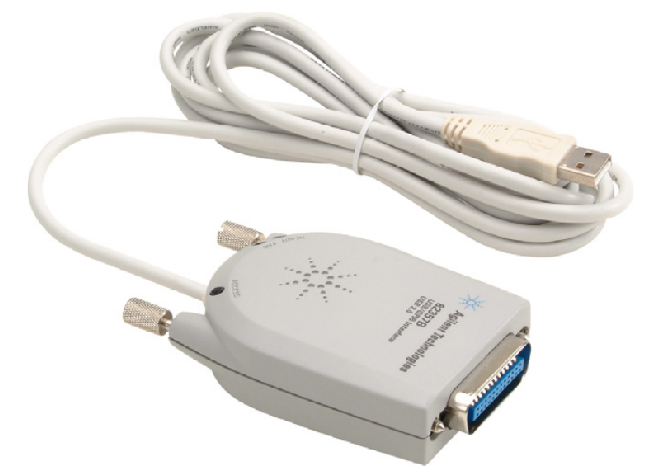
\includegraphics[width=10cm]{Imagenes/AdaptadorGpibUsb.pdf}
				\caption{Adaptador USB GPIB 82357B de Agilent Technologies}
				\label{Fig:AdaptadorGpibUsb}
			\end{center}
		\end{figure}	
		
		La empresa \emph{Keysight Technologies} (antigua Agilent) proporciona un conjunto de herramientas de software, conocido bajo el nombre de \emph{IO Libraries Suite}, de libre descarga en el sitio web de esta empresa en la versión 6.2017, a la fecha de redactar esta nota.
		
		IO Libraries Suite proporciona el software necesario para el intercambio de datos con instrumentos programables a través de buses RS232, GPIB, USB y redes LAN. El software se presenta en forma de utilidades ejecutables que permiten enviar comandos a los instrumentos y recibir sus respuesta, resolución de problemas así como también un librerías para desarrollo de aplicaciones.
		
		Las librerías \emph{VISA (Virtual Instruments Software Architecture) } proporcionan una capa de software uniforme desde el punto de vista del programador, para el acceso a los buses mencionados. La librería VISA es parte integral de \emph{IO Libraries Suite}. Existen librerías VISA producidas por otras empresas del ramo de la instrumentación inteligente, una de las más reconocidas es la librería \emph{VISA de National Instruments (NI-VISA)} así como también la librería VISA de Tektronix.
		
		El software proporcionado por Keysight Technologies es exclusivo para ambiente Windows. Las librerías VISA de National Instruments están dirigidas Windows y a ciertas distribuciones de Linux, pero no para Ubuntu.
		
		Existe una alternativa, la librería \emph{linux-gpib} 
		
		Para utilizar el dispositivo adaptador USB / GPIB se requiere el siguiente soporte de software
		
		\begin{itemize}
			\item El soporte a nivel de librerías de usuario (user space) en el PC, en Ubuntu se recurre a \emph{linux-gpib}.
			\item El soporte de software a nivel de núcleo de sistema (kernel)en el PC, los módulos de núcleo.
			\item El soporte a nivel de firmware en el dispositivo Agilent 82357B, es necesario cargar una versión actualizada del firmware para este dispositivo.
		\end{itemize}
	
		\subsection{Instalación de linux-gpib y módulos de núcleo}
		
		La librería \texttt{linux-gpib} se construirá a partir de su código fuente, el cual puede descargarse de forma libre en el siguiente enlace,
		
		\begin{link}
			https://sourceforge.net/projects/linux-gpib/?source=dlp
		\end{link}
		
		Como requisito para construir esta librería, en el sistema deben estar instalados los archivos de cabecera del núcleo, apropiado para la versión de núcleo de linux que se este utilizando. El comando \texttt{uname} de shell de linux permite obtener la versión de núcleo que se este utilizando,
		
		\begin{code}
			uname -r
		\end{code}
		
		Por medio del siguiente comando de shell se instalan los archivos de cabecera, acordes a la versión de linux,
		
		\begin{code}
			sudo apt-get update		\\
			sudo apt-get install linux-headers-\$(uname -r)
		\end{code}
		
		Si se desea tener acceso a esta librería por medio de Python, se debe instalar el paquete \texttt{python-setuptools},
		\begin{code}		
			sudo apt-get install python-dev libboost-python-dev python-setuptools --yes
		\end{code}
			
		Ahora se procede a la descarga de los archivos fuente para la librería \texttt{linux-gpib}, puede hacerse sin salir del shell por medio del comando \texttt{wget}. Se puede crear un directorio nuevo para almacenar los archivos descargados, ejecutando previamente \texttt{mkdir nombre\_directorio}.
		
		\begin{code}
			wget --content-disposition --no-check-certificate \\
			https://sourceforge.net/projects/linux-gpib/files/latest/download?source=dlp
		\end{code}
		
		El paso siguiente es descomprimir el archivo mediante el comando de shell \texttt{tar}, como se indica a continuación, en donde se debe introducir el nombre del archivo comprimido el cual indica la versión, en este caso se trata de la versión 3.2.20,

		\begin{code}		
			tar xvfz tar xvfz linux-gpib-3.2.20.tar.gz
		\end{code}
			
		Ahora se procede a construir la librería, por medio de la secuencia de comandos,
		
		\begin{code}		
			./configure \\		
			make -j8 	\\		
			make install
		\end{code}
					
		Para comprobar que la librería ha sido instalada correctamente, el comando de shell \texttt{whereis} nos reporta la ubicación del la librería \texttt{libgpib.so}.
		
		\begin{code}
			whereis libgpib.so
		\end{code}
		
		La repuesta del comando debe indicar la ruta en donde se encuentra la librería. En Debian:

		\begin{code}		
			libgpib: /usr/local/lib/libgpib.so /usr/local/lib/libgpib.la
		\end{code}
	
		\subsection{Instalación de módulos de núcleo}
		
		El módulo de núcleo llamado \texttt{agilent\_82357a.ko} también fue instalado durante el procedimiento de construcción e instalación del código fuente en el paso anterior. Para proceder a su carga, se debe ubicar este módulo dentro del sistema de archivos. Por ejemplo, en Debian, se encuentra en \texttt{/lib/modules/3.16.0-4-amd64/gpib/agilent\_82357a}. En esta ruta el subdirectorio con nombre \texttt{3.16.0-4-amd64} indica la versión de núcleo del PC (3.14) y su arquitectura (amd64). 
		
		Nos ubicaos dentro de la carpeta que contiene este módulo, para proceder a su carga con el comando de shell \texttt{modprobe}, de la siguiente forma,
		
		\begin{code}
			sudo modprobe agilent\_82357a
		\end{code}
		
		Si la carga ocurre de forma correcta, el comando no genera ninguna repuesta. Así que se debe revisar si el módulo ha sido cargado de forma adecuada, por medio de los siguientes comandos de shell,
		
		\begin{code}		
			lsmod | grep agilent
		\end{code}
	
		Este comando emite una repuesta similar a la siguiente,

		\begin{code}
			agilent\_82357a	22661  0 \\				
			gpib\_common	35582  1 agilent\_82357a  \\				
			usbcore	195468  4 uhci\_hcd,agilent\_82357a,ehci\_hcd,ehci\_pci \\
		\end{code}
		
		La primera línea de la salida del comando \texttt{lsmod} indica que el módulo \texttt{agilent\_82357a} se ha cargado correctamente. 	
		
		El comando de shell \texttt{modinfo} permite obtener información sobre un módulo, se puede utilizar para verificar que el modulo \texttt{agilent\_82357a} ha sido cargado, 
		
		\begin{code}
			modinfo agilent_82357a 			
		\end{code}
		
		Al ejecutar el comando anterior, se obtiene un respuesta similar a la siguiente,
		
		\begin{code}
			filename:    /lib/modules/3.13.0-110-generic/gpib/agilent\_82357a/ \\ agilent\_82357a.ko \\
			license:        GPL \\
			srcversion:     BAB8466E207C02D6E8023B3 \\
			alias:          usb:v0957p0718d*dc*dsc*dp*ic*isc*ip*in* \\
			alias:          usb:v0957p0107d*dc*dsc*dp*ic*isc*ip*in* \\
			depends:        gpib\_common \\
			vermagic:       3.13.0-110-generic SMP mod\_unload  modversions 686 
		\end{code}
	
		La cual indica que el módulo ha sido cargado correctamente.
		
		\subsection{Instalación de archivos binarios de firmware para el 82357B}	
		
		Para que el dispositivo 82357B funcione correctamente debe actualizarse su firmware. Los archivo binarios para el firmware se pueden descargar en el siguiente enlace, 
		
		\begin{link}
			http://linux-gpib.sourceforge.net/firmware/gpib\_firmware-2008-08-10.tar.gz
		\end{link}
	
		Se descargan los binarios comprimidos, se descomprimen con los acostumbrados comandos \texttt{wget} y \texttt{tar} respectivamente,
		
		\begin{code}
			wget https://gist.github.com/turingbirds/6eb05c9267a6437183a9567700e8581a \\ 		
			tar xvfz gpib\_firmware-2008-08-10.tar.gz 
		\end{code}
		
		Se necesita la utilidad de linux \texttt{fxload} que permite cargar en un dispositivo USB un archivo de firmware con extensión \texttt{.hex}. La utilidad \texttt{fxload} se construirá a partir de su código fuente, éste se descarga mediante el siguiente enlace,
		
		\begin{link}		
			https://downloads.sourceforge.net/project/linux-hotplug/fxload/ \\ 2008\_10\_13/fxload-2008\_10\_13.tar.gz		
		\end{link}
		
 		Siguiendo un procedimiento similar al mostrados anteriormente, se descarga el archivo comprimido, se descomprime para luego construir el código fuente de la forma acostumbrada en entornos linux. 
		
		Se descarga de este enlace el código fuente con el comando de shell \texttt{wget},
		
		\begin{code}			
			wget --content-disposition --no-check-certificate \\ https://downloads.sourceforge.net/project/linux-hotplug \\ /fxload/2008\_10\_13/fxload-2008\_10\_13.tar.gz
		\end{code}
		
		Se descomprime el archivo con el comando de shell \texttt{tar},

		\begin{code}				
			tar xvfz fxload-2008\_10\_13.tar.gz
		\end{code}
	
		Ahora se ingresa al subdirectorio \texttt{fxload-2008\_10\_13} en donde se encuentra el códifo fuente,

		\begin{code}			
			cd fxload-2008\_10\_13
		\end{code}
		
		Se construye el mismo por medio de los comandos,
		
		\begin{code}	
			make	\\		
			sudo make install
		\end{code}
		
		Se deben editar tres lineas en el archivo \texttt{/etc/gpib.conf}. Se emplea el editor de archivos \texttt{nano} como super usuario, de la siguiente forma, 
		
		\begin{code}			
			sudo nano /etc/gpib.conf
		\end{code}
		
		Dentro del archivo \texttt{gpib.conf} se editan las líneas que contienen las entradas para \texttt{board\_type}, \texttt{name} y \texttt{pad}. Para la entrada \texttt{name} el usuario puede introducir una cadena descriptiva, sin espacios, para identificar el adaptador. La entrada \texttt{pad} indica la dirección primaria del adaptador GPIB, el usuario puede establecer un valor numérico entre 0 y 30.
		
		\begin{code}	
			board\_type = ``agilent\_82357a" \\		
			name = ``AGILENT82357B" \\		
			pad = 22
		\end{code}
		
		Prosigue la carga de los módulos de núcleo que le dan soporte al adaptador 82357B, \texttt{gpib\_common} y \texttt{agilent\_82357a} se cargan por medio del comando shell \texttt{modprobe} de la siguiente forma,
		
		\begin{code}
			sudo modprobe gpib\_common \\		
			sudo modprobe agilent\_82357a
		\end{code}
		
		Ahora se procede a insertar el dispositivo 82357B en el puerto USB del PC, en éste solo debe encontrarse iluminado en rojo el led etiquetado como LED FAIL. 
		
		Por medio del comando \texttt{lsusb} se encuentran los identificadores (ID) de bus (\emph{bus ID}) y de dispositivo (\emph{device ID}), dentro de la ventana de shell se ejecuta,
		
		\begin{code}
			lsusb
		\end{code}
		
		El comando arroja varias entradas como respuesta, en una de ellas se debe encontrar la entrada para el adaptador de Agilent Technologies, similar a la que se muestra a continuación,
	
		\begin{code}
			Bus 002 Device 005: ID 0957:0518 Agilent Technologies, Inc.
		\end{code}
		
		De esta linea se infiere que el ID de bus es el valor 002 y el ID de dispositivo es el valor 005. Los valores de ID de bus y ID de dispositivo pueden resultar diferentes, dependiendo del equipo donde se ejecute el comando. Se requieren estos datos en los argumentos del comando \texttt{fxload}.
		
		Dentro de los archivos de firmware descargados se encuentra el archivo llamado \texttt{measat\_releaseX1.8.hex}, que contiene el firmware para el dispositivo. Para cargar el firmware en el dispositivo 82357B se emplea la utilidad de shell \texttt{fxload} ejecutada como superusuario, 
		
		\begin{code}
			sudo fxload -D /dev/bus/usb/002/005  -t fx2 -I \\ gpib\_firmware-2008-08-10/agilent\_82357a/measat\_releaseX1.8.hex
		\end{code}
		
		En el dispositivo 82357B el LED FAIL debe estar aún iluminado en rojo. Se debe proceder a una nueva carga del firmware. Por medio del comando \texttt{lsusb} se obtienen por segunda vez el ID de bus y el ID de dispositivo
		
		\begin{code}
			lsusb
		\end{code}
	
		El comando debe generar una respuesta similar a la siguiente,
		
		\begin{code}
			Bus 002 Device 006: ID 0957:0518 Agilent Technologies, Inc.
		\end{code}
		
		El ID de bus debe ser el mismo (Bus 002), el valor que debería haber cambiado es el ID de dispositivo (que ahora es Device 006). Se procede nuevamente a ejecutar la utilidad \texttt{fxload}, introduciendo en el argumento de este comando el valores de ID de bus y el nuevo valor de ID de dispositivo,
		
		\begin{code}
			sudo fxload -D /dev/bus/usb/002/006  -t fx2 -I \\ gpib\_firmware-2008-08-10/agilent\_82357a/measat\_releaseX1.8.hex
		\end{code}
		
		Como resultado de la ejecución del comando, en el dispositivo 82357B todos los LEDs deben encontrarse encendidos.		
		
		Se deben cambiar los permisos sobre el archivo que representa al dispositivo USB / GPIP, ubicado en la ruta \texttt{/dev/gpib0}, por medio del comando,
		
		\begin{code}
			sudo chmod 666 /dev/gpib0
		\end{code}
		
		Resta inicializar el dispositivo 82357B por medio del comando de shell \texttt{gpib\_config}. Este comando tiene ciertos problemas en ubicar la librería \texttt{libgpib.so}, así que se debe crear un \emph{enlace simbólico} hacia ésta, de la siguiente forma,
		
		\begin{code}
			sudo ln -s /usr/local/lib/libgpib.so.0 /lib/libgpib.so.0
		\end{code}
		
		Para ahora ejecutar el comando
			
		\begin{code}
			\texttt{gpib\_config}
		\end{code}
	
		Como resultado de procedimiento en el dispositivo 82357B se debe encontrar únicamente el LED READY iluminado en verde.
			
	\section{Anexos}	
		
	\subsection{Script de Bash para carga automática de firmware}
	
	\begin{lstlisting}[language=bash,caption={bash version}]
#!/bin/bash 

# Script de Bash para actualización automatica de firmware para 
# el adaptador USB a GPIB Agilent 82357B.
# Se encarga de buscar el ID de BUS y el ID de DEVICE para 
# preparar el comando de carga de fimware, por medio de <fxload>. 
# El comando de carga debe ejecutarse dos veces, debido a un bug 
# en el archivo .hex de codigo de firmware.

# Autor: 	Jose A. Arias B.
# Correo: 	correo@josearias.com.ve
# Version:	1.0

re="Bus ([0-9]+) Device ([0-9]+): ID 0957:0518"
#input="Bus 001 Device 006: ID 0957:0518 Agilent Technologies, Inc."

input=$(lsusb)

if [[ $input =~ $re ]] 
then 

	echo "Encontrado adaptador Agilent 82357B"
	echo "Primer intento para carga de firmware"

	bus=${BASH_REMATCH[1]}
	dev=${BASH_REMATCH[2]}
	echo ${BASH_REMATCH[0]}
	echo "1: Bus = $bus Device = $dev"
	sudo fxload -D /dev/bus/usb/$bus/$dev  -t fx2 -I 
	 /etc/hotplug/usb/agilent_82357a/measat_releaseX1.8.hex

else 

	echo "No se ha encontrado al adaptador Agilent 82357B"
	exit

fi
# Espera a que proceda la carga de firmware
sleep 3

input=$(lsusb)
echo $input

if [[ $input =~ $re ]]
then

echo "Segundo intento para carga de firmware"
bus=${BASH_REMATCH[1]}
dev=${BASH_REMATCH[2]}
echo ${BASH_REMATCH[0]}
echo "2: Bus = $bus Device = $dev"
sudo fxload -D /dev/bus/usb/$bus/$dev  -t fx2 -I
 /etc/hotplug/usb/agilent_82357a/measat_releaseX1.8.hex

# Espera de nuevo a que proceda la carga de firmware
sleep 3

sudo gpib_config

fi

echo "El adaptador Agilent 82357B esta listo para usarse"
	\end{lstlisting}	

		
\end{document}